\pagestyle{plain}

\subsection{TEM images}\label{TEM_images}

TEM samples were prepared and TEM images were acquired. Various shapes and sizes of nanoparticles and nanorods were used. There were two samples of nanorods with unknown size and four sizes of nanoparticles with diameters 20 nm, 40 nm, 50 nm and 80 nm. There are examples of 20 nm nanoparticles (fig:\ref{fig:20nm}), 40 nm nanoparticles (fig:\ref{fig:40nm}) and nanorods (fig:\ref{fig:NRs}) with absorption peak on wavelength 800 nm.

\begin{figure}[h!]
\begin{center}
    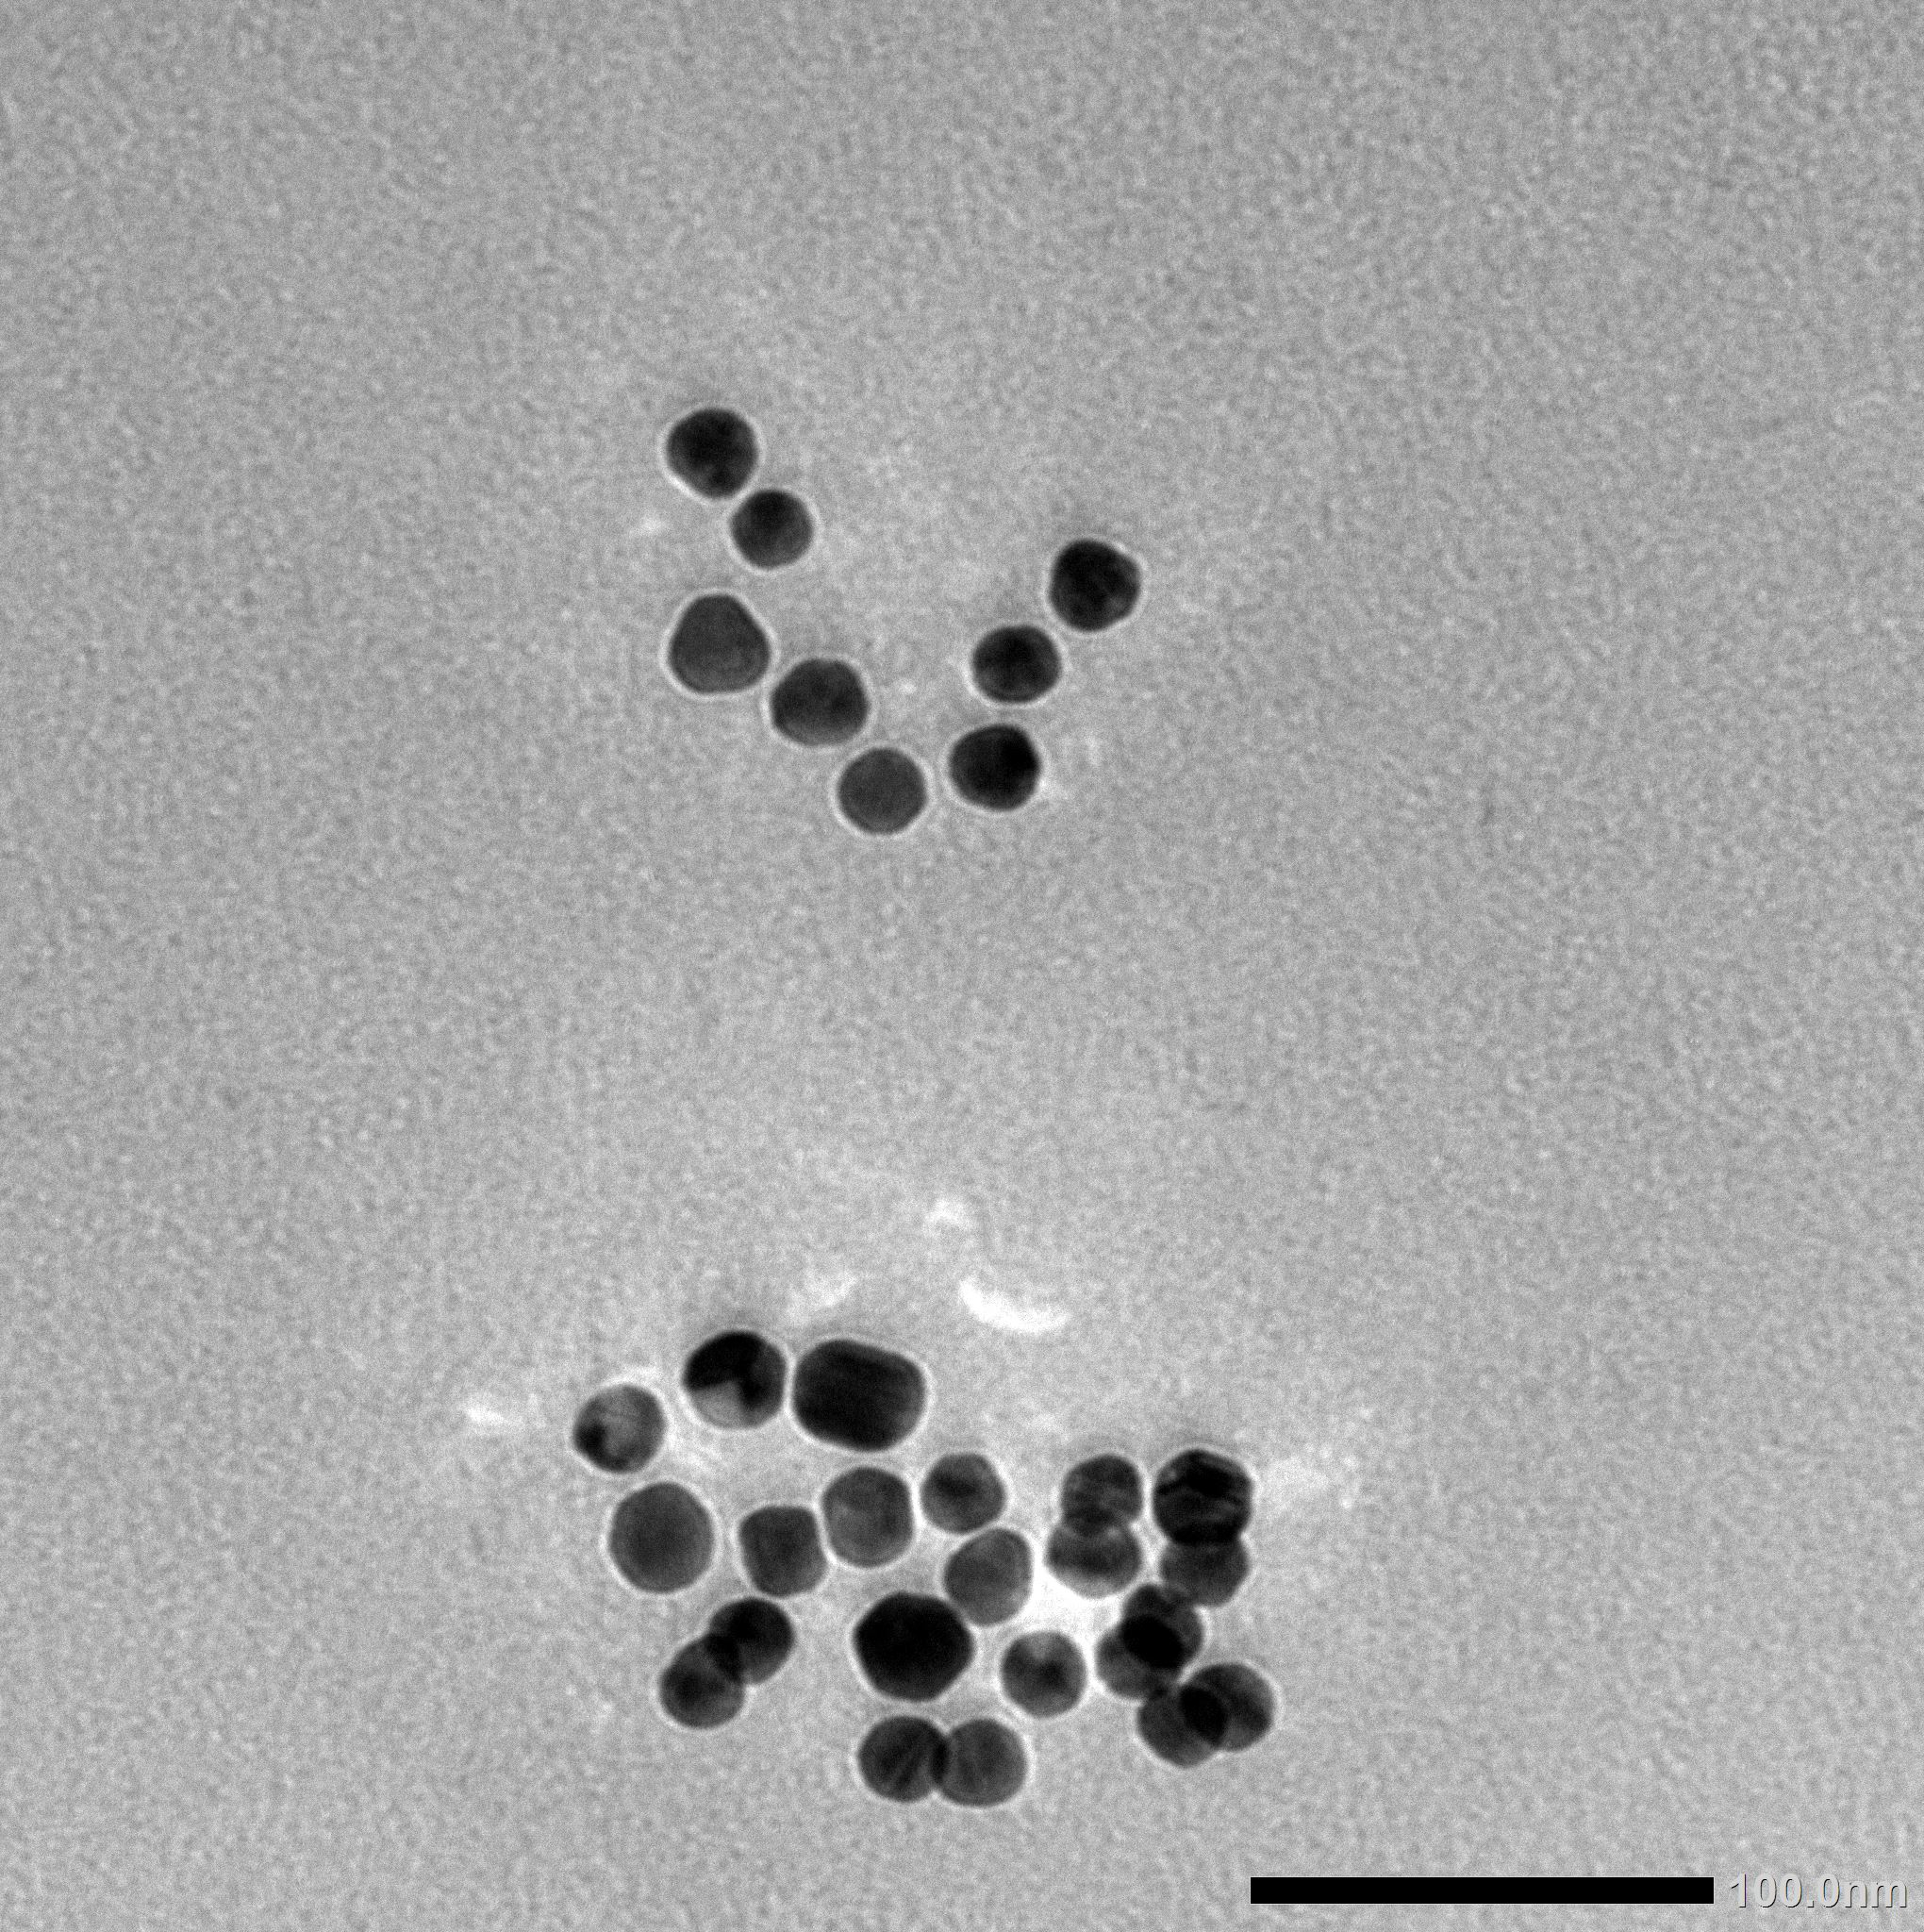
\includegraphics[width=0.5\linewidth]{20nm.jpg}
    \caption{Raw TEM image of 20 nm nanoparticles}~\label{fig:20nm}
\end{center}
\end{figure}

\begin{figure}[h!]
\begin{center}
\begin{subfigure}(a)
    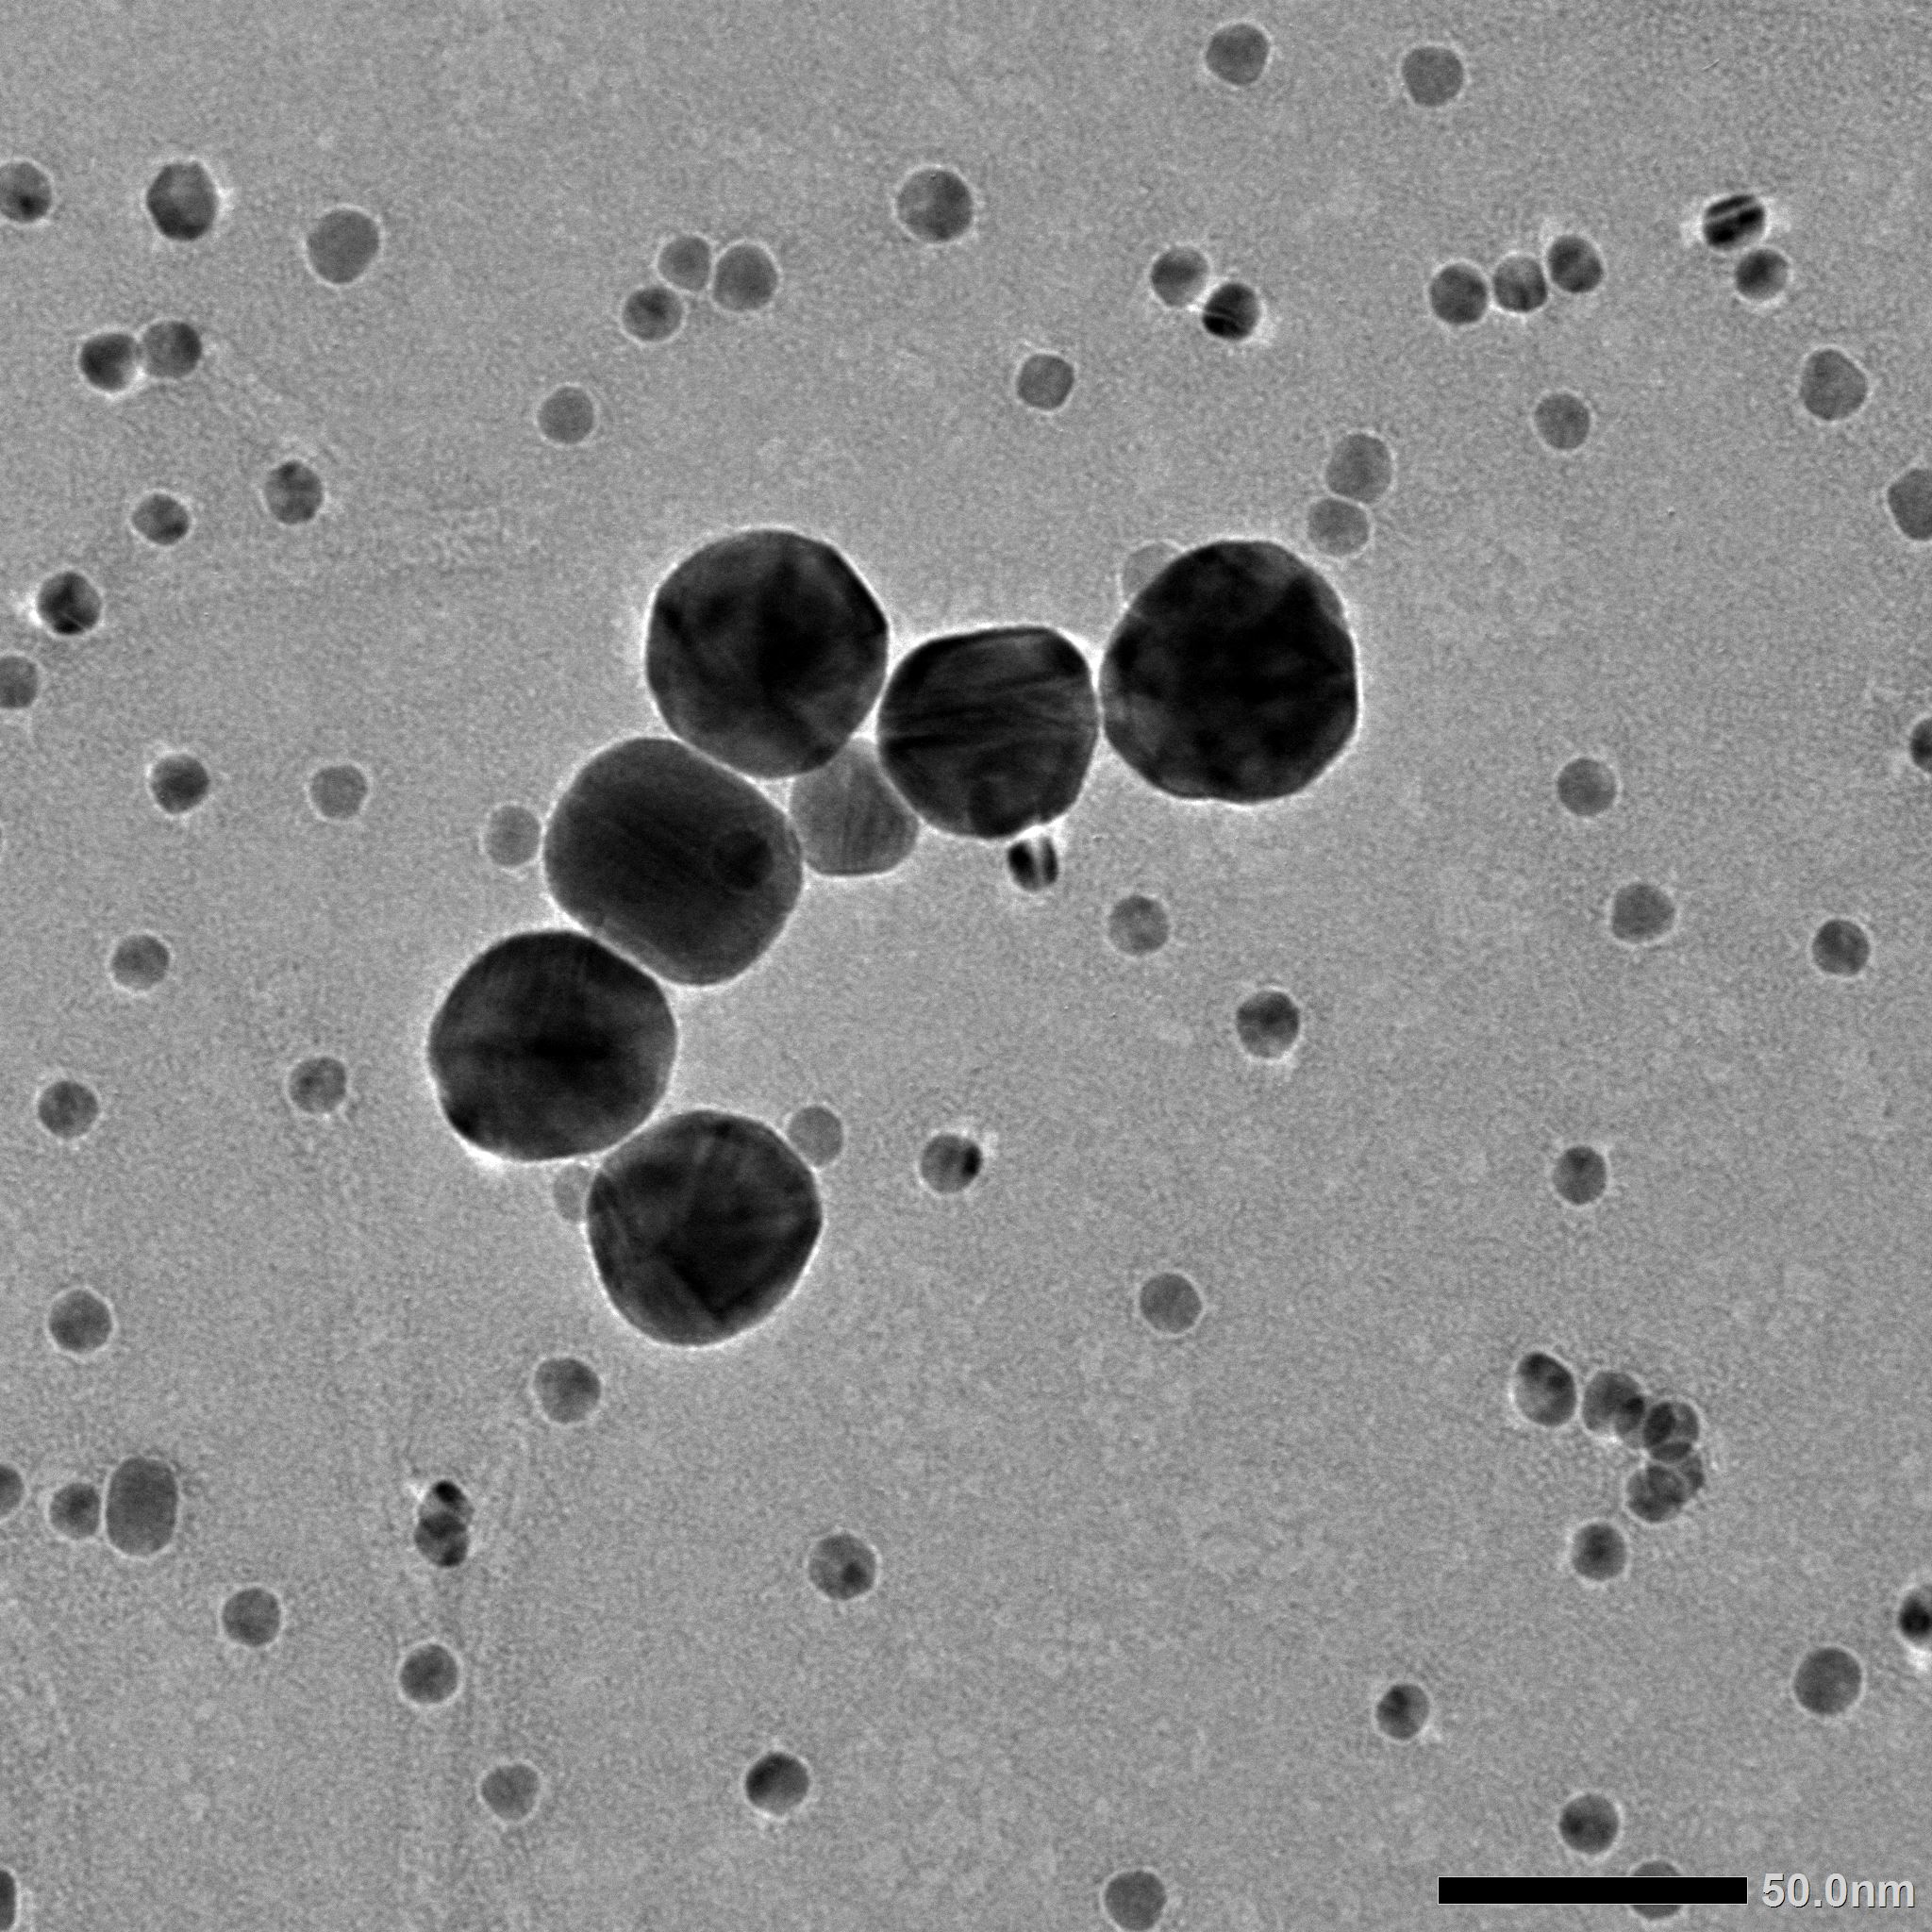
\includegraphics[width=0.4\linewidth]{40nm.jpg}
\end{subfigure}
\begin{subfigure}(b)
    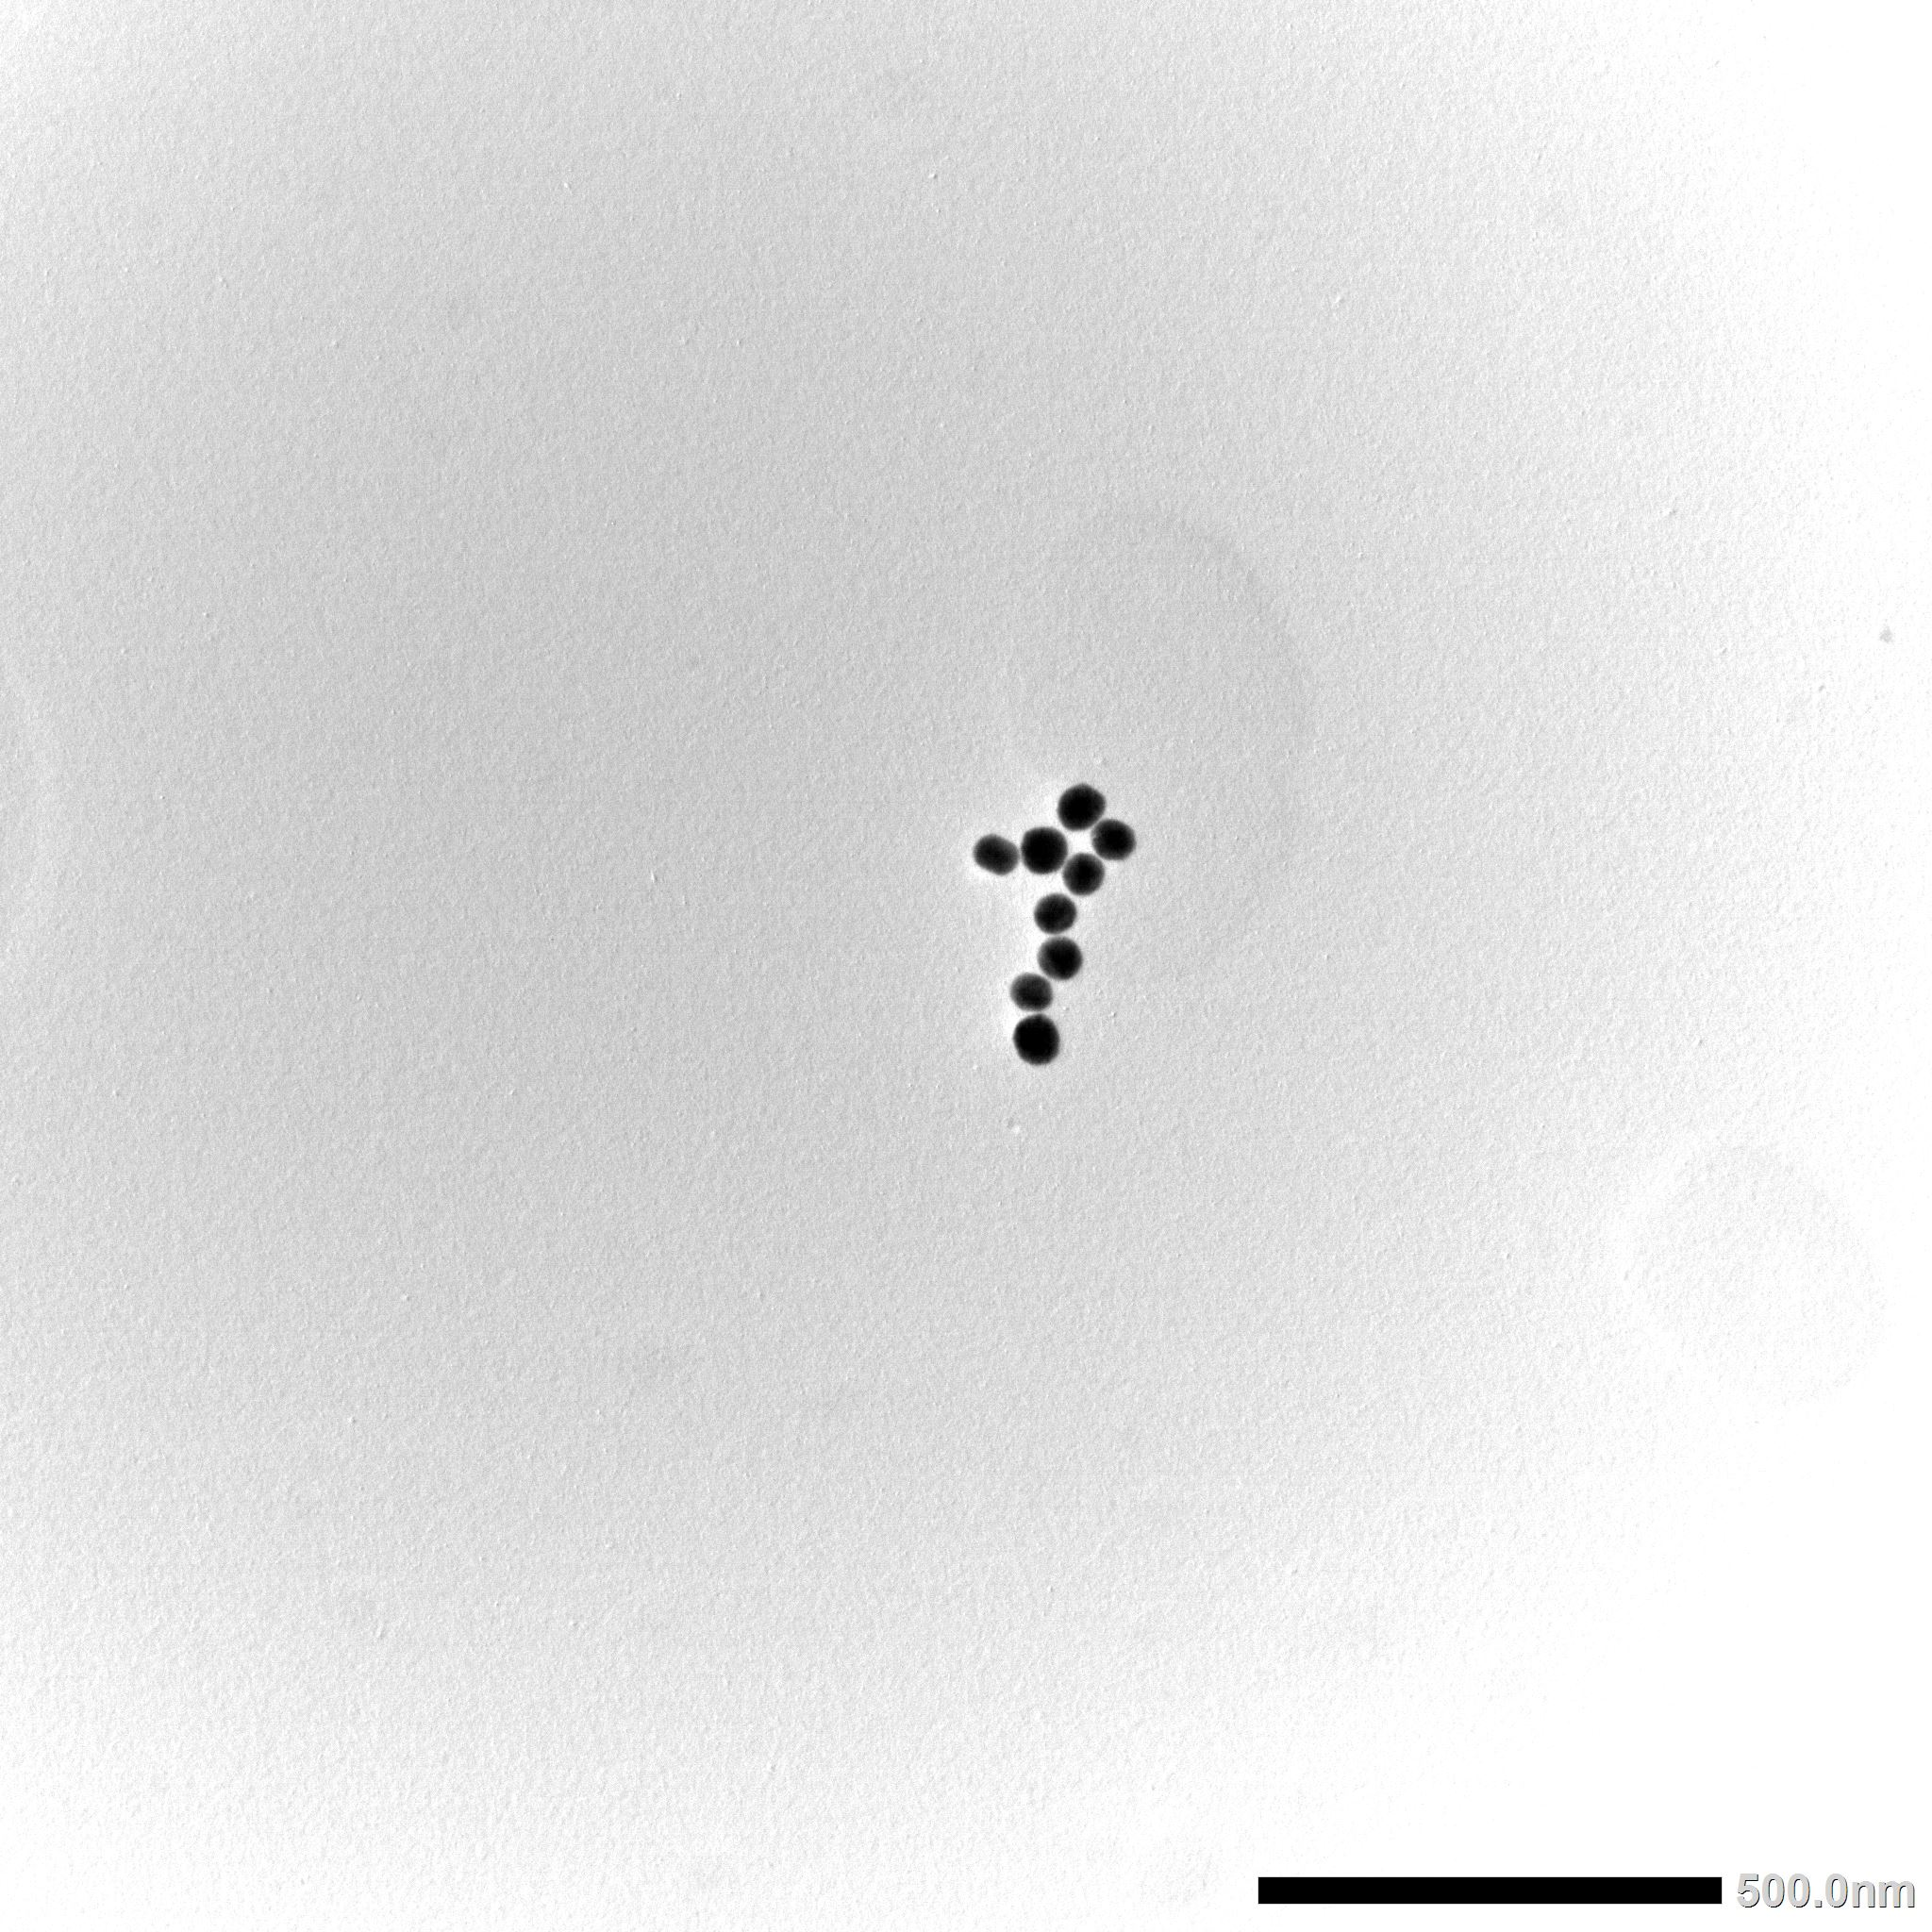
\includegraphics[width=0.4\linewidth]{50nm.jpg}
\end{subfigure}
\caption{Raw TEM images of 40 nm (a) and 50 nm (b) nanoparticles}~\label{fig:40nm}
\end{center}
\end{figure}

\begin{figure}[h!]
\begin{center}
\begin{subfigure}(a)
    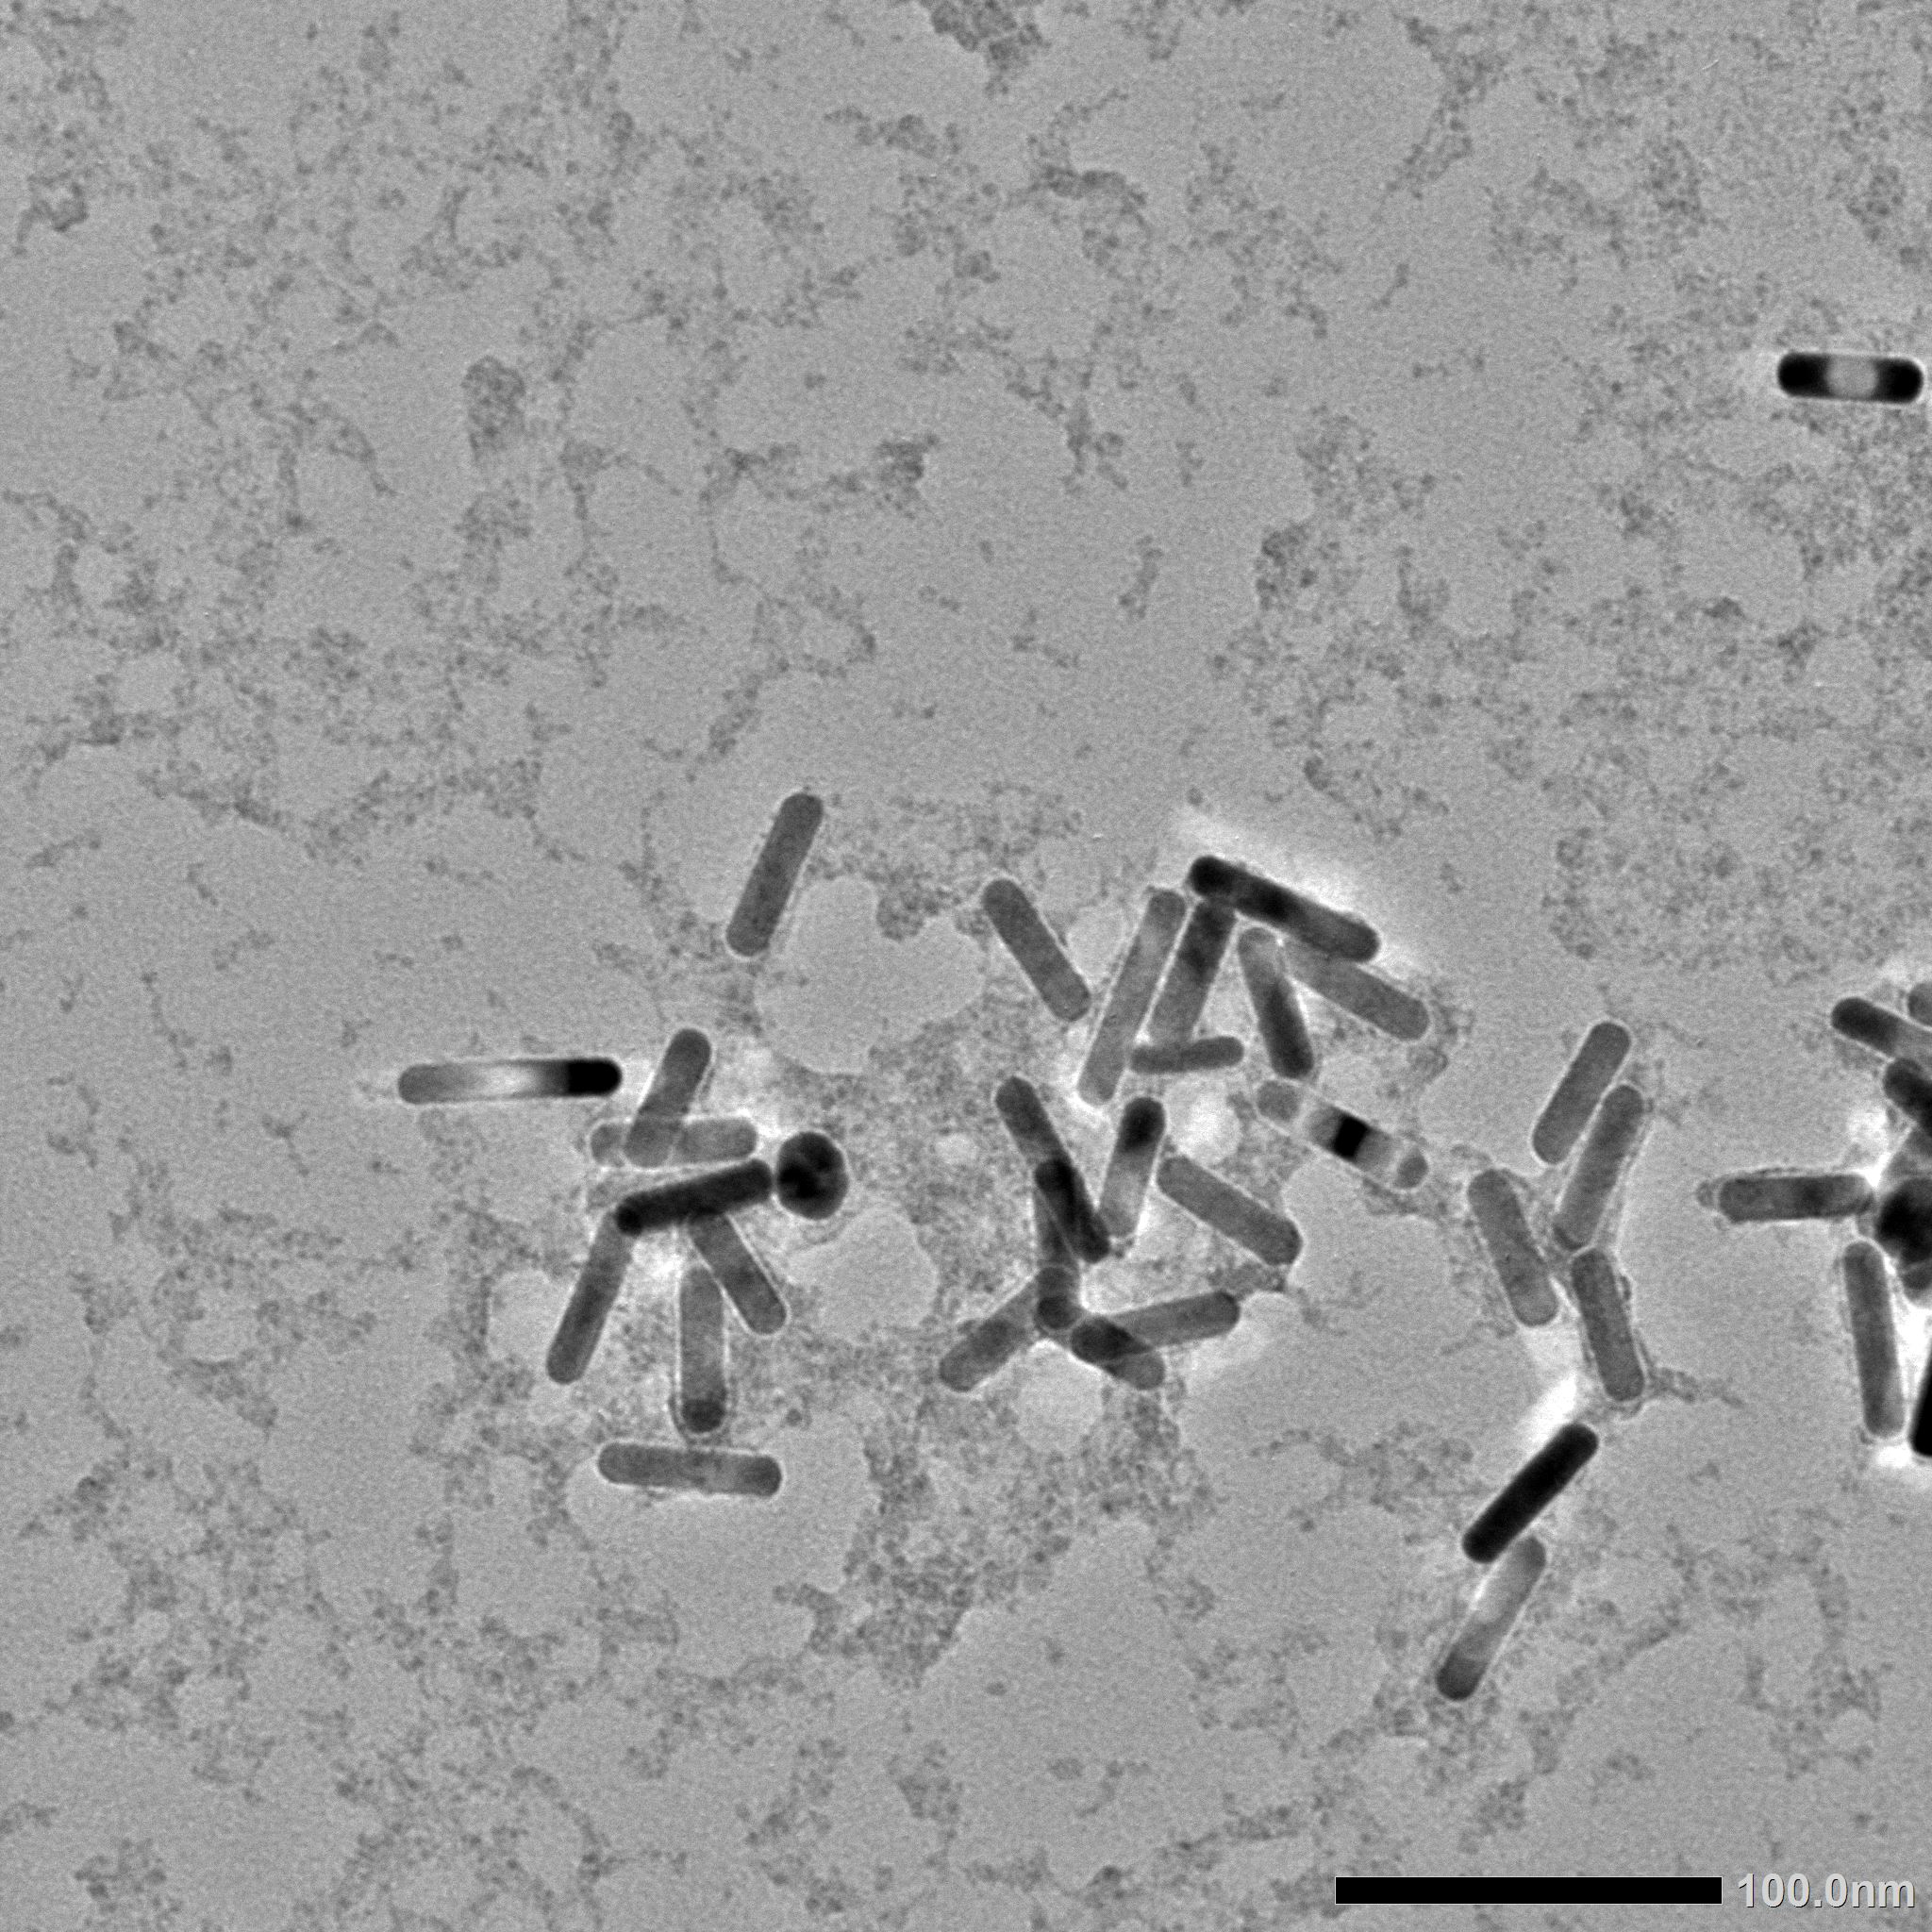
\includegraphics[width=0.4\linewidth]{NRs.jpg}
\end{subfigure}
\begin{subfigure}(b)
    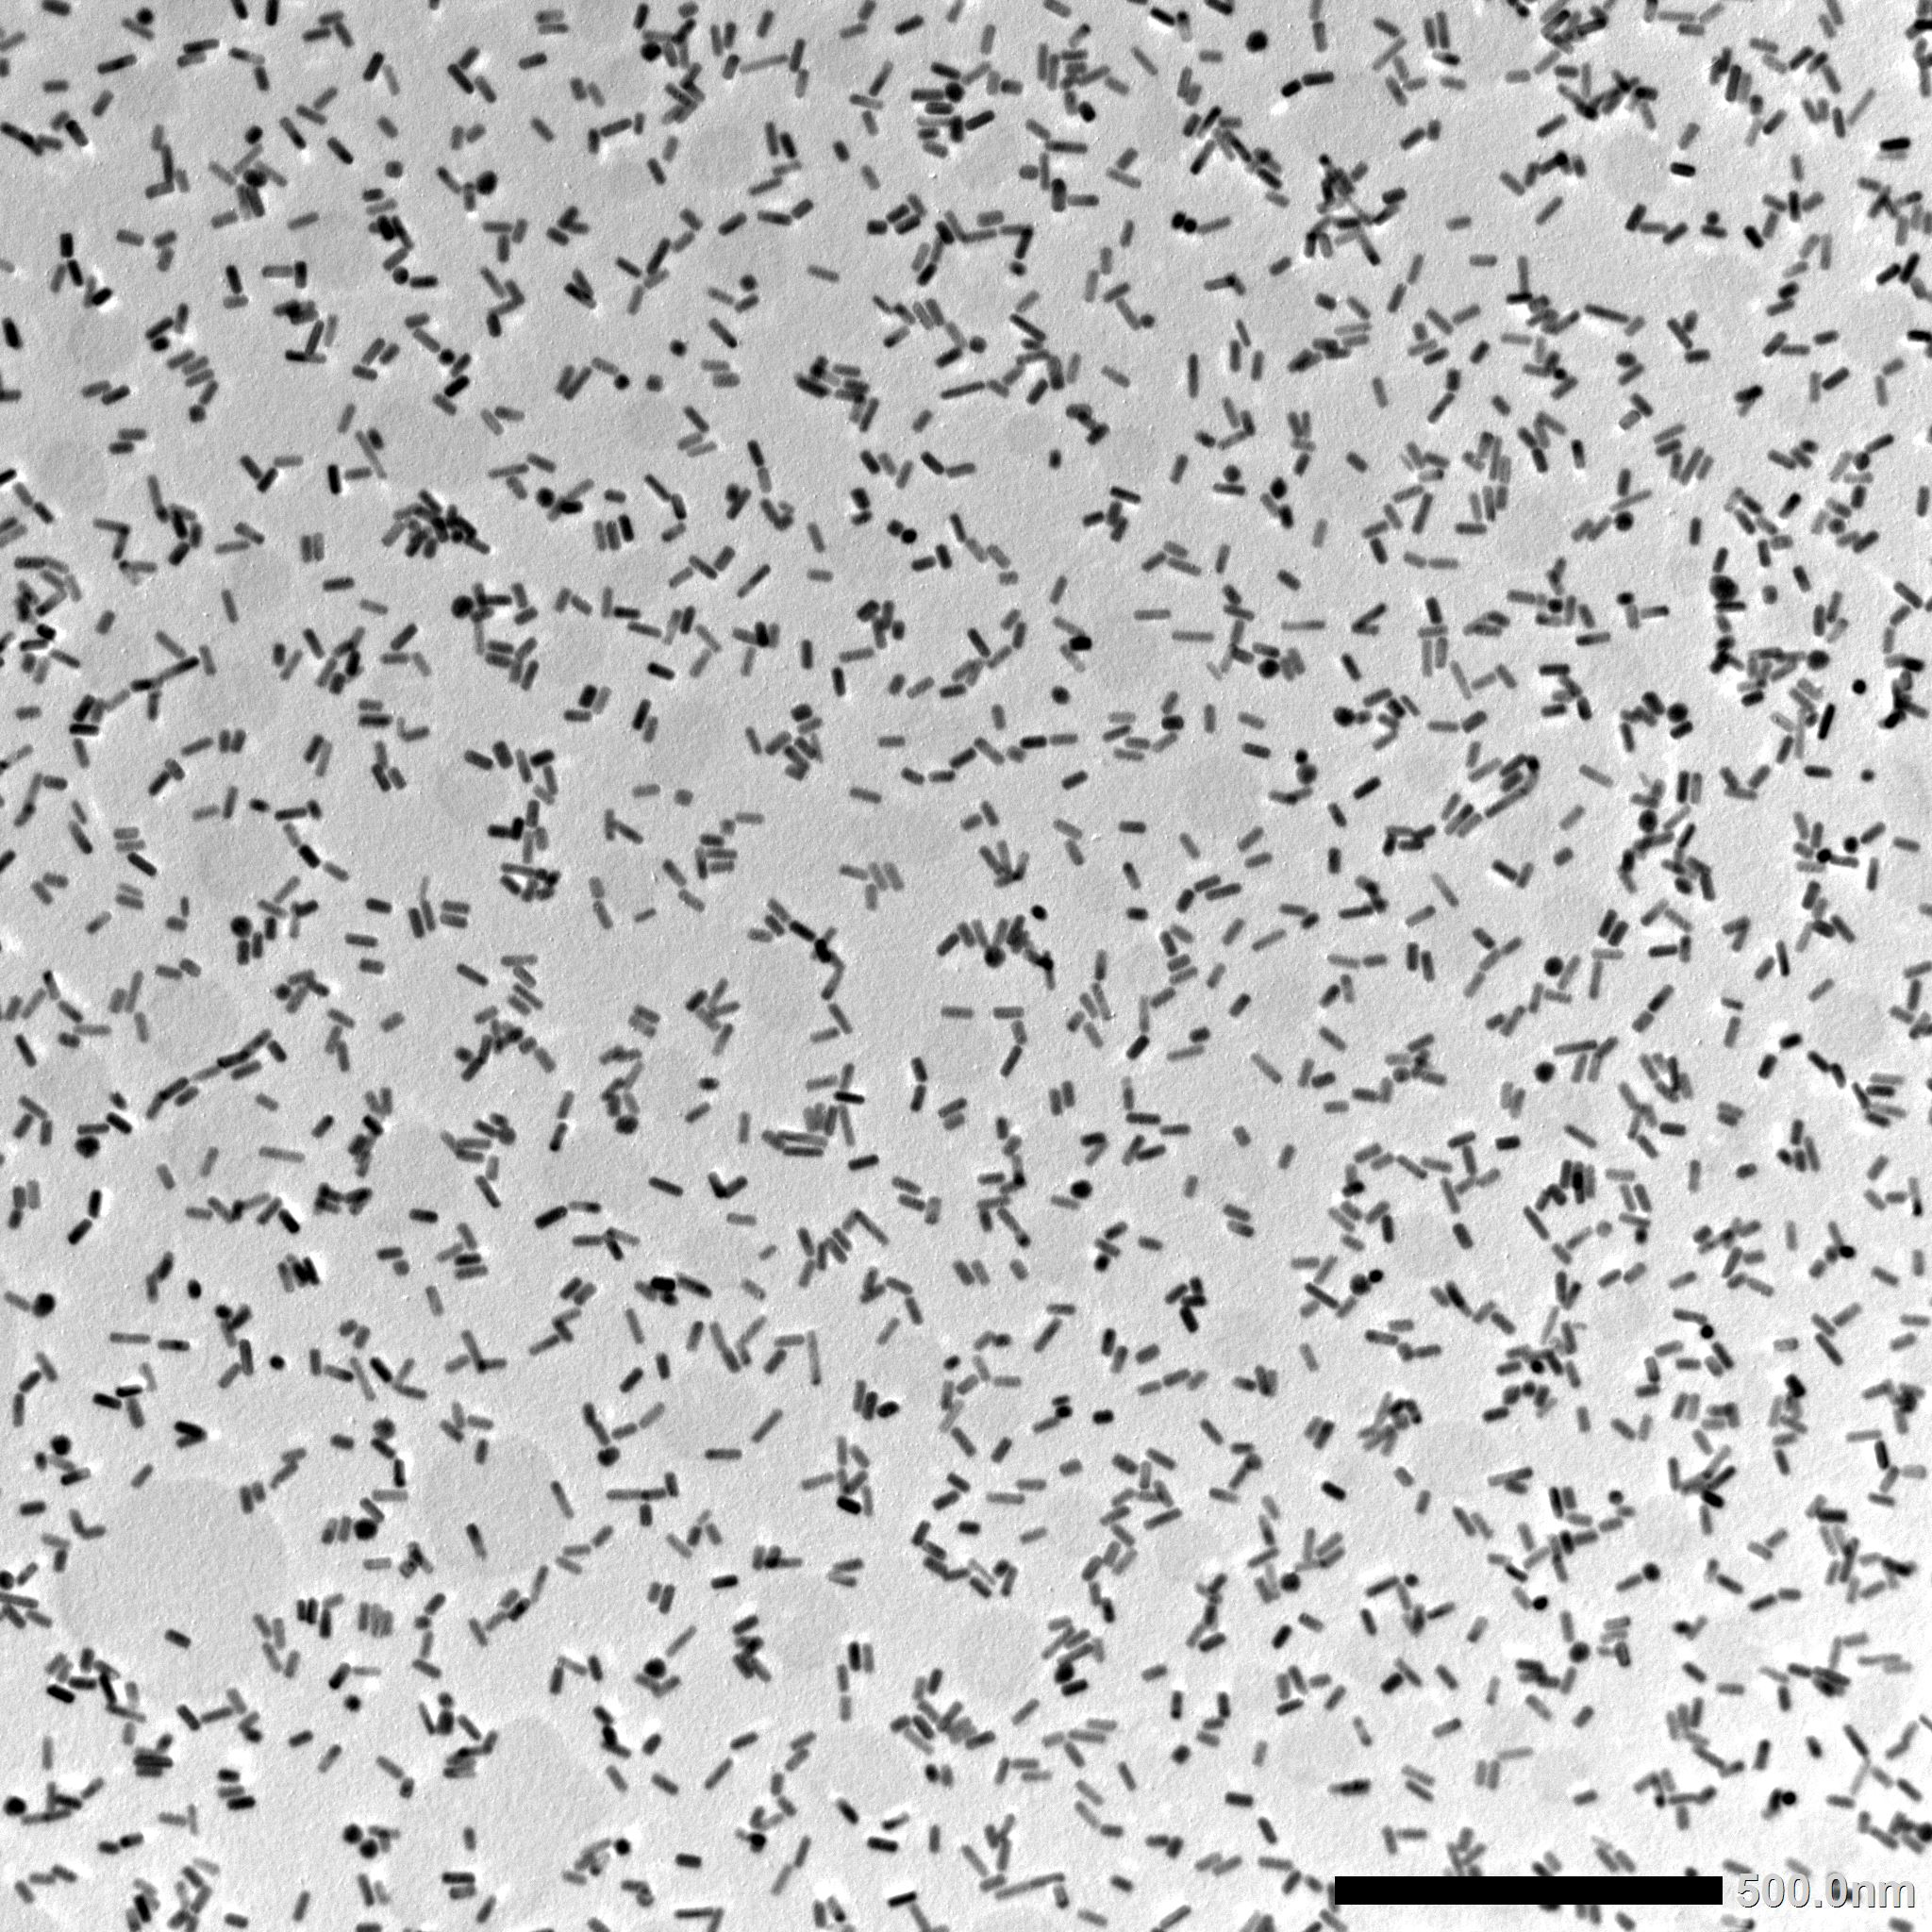
\includegraphics[width=0.4\linewidth]{NRs2.jpg}
\end{subfigure}
\caption{Raw TEM images of nanorods}~\label{fig:NRs}
\end{center}
\end{figure}

\subsection{Python program}\label{program}

Python program was created (see Attachement). Program is able to process more images at once and it can run from command line with arguments, user may define folder with images or decide if results should be plotted or not. Program requires metadata in json format, which includes information about type of particles (nanoparticles or nanorods) and scale of TEM image. Program perform image segmentation and returns labeled images, average sizes and histograms of sizes.

\subsection{Program outputs}\label{outputs}

Program was tested with various input data, examples of results can be seen on figures \ref{fig:res20nm}, \ref{fig:res40nm} and \ref{fig:resNRs}.

\begin{figure}[h!]
\begin{center}
    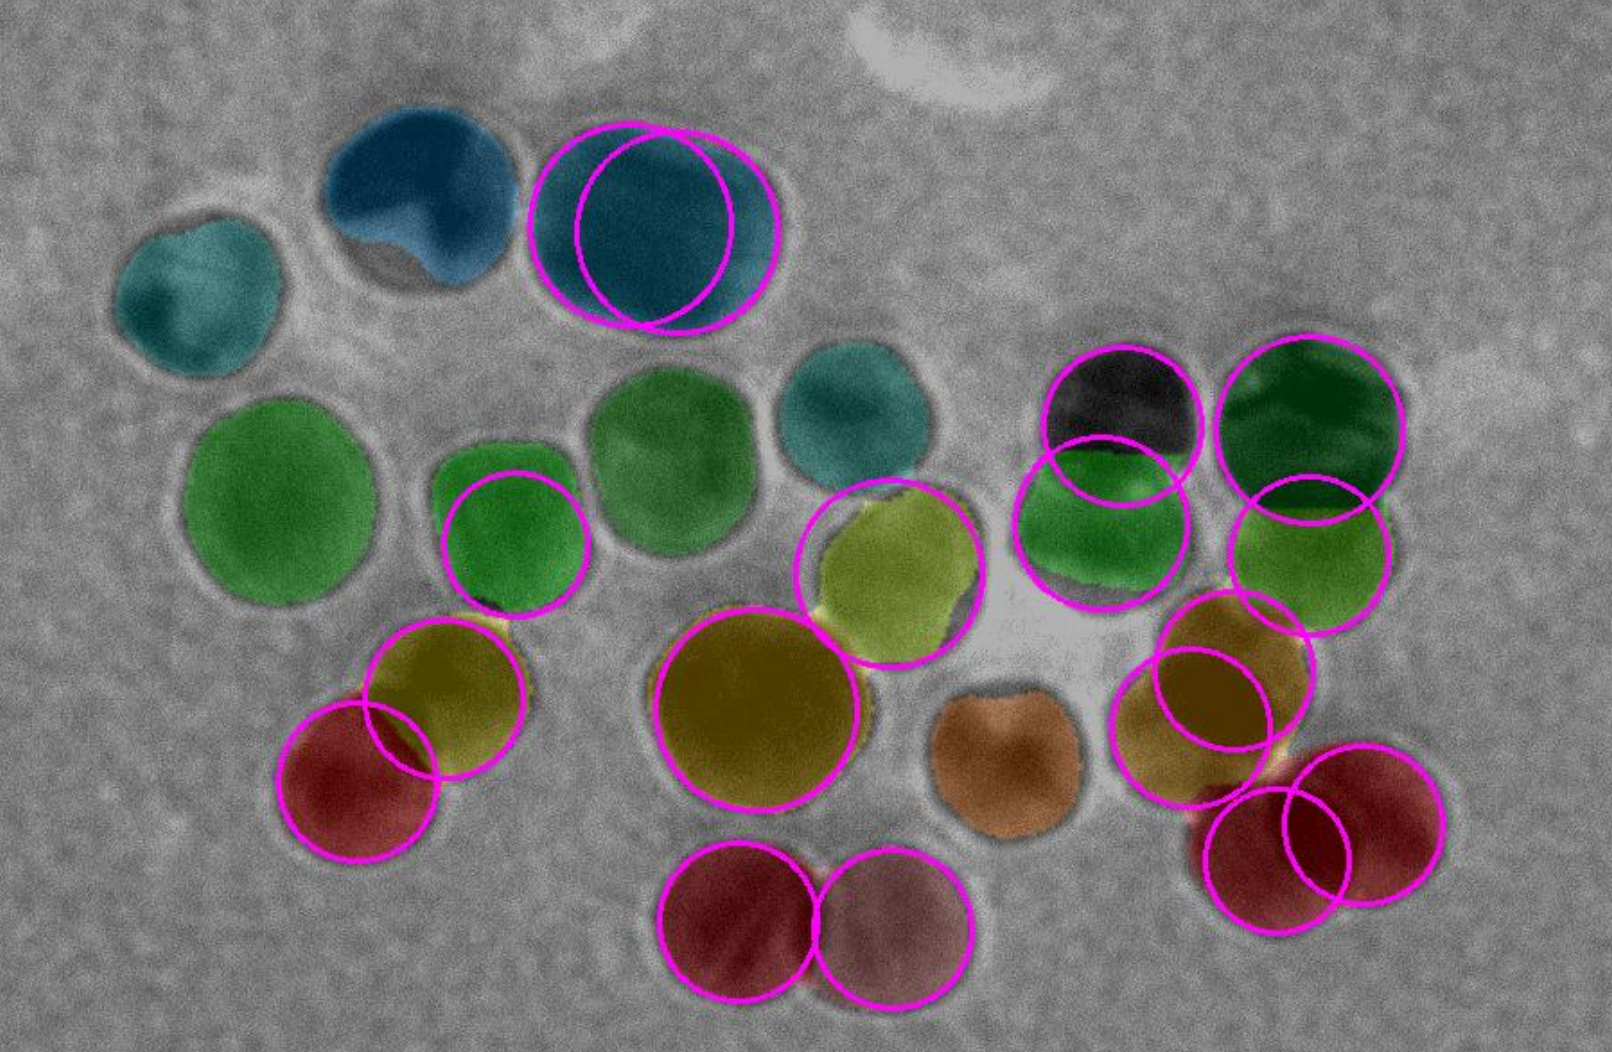
\includegraphics[width=0.5\linewidth]{res20nm.png}
    \caption{Croped result labeled image of 20 nm nanoparticles}~\label{fig:res20nm}
\end{center}
\end{figure}

\begin{figure}[h!]
\begin{center}
\begin{subfigure}(a)
    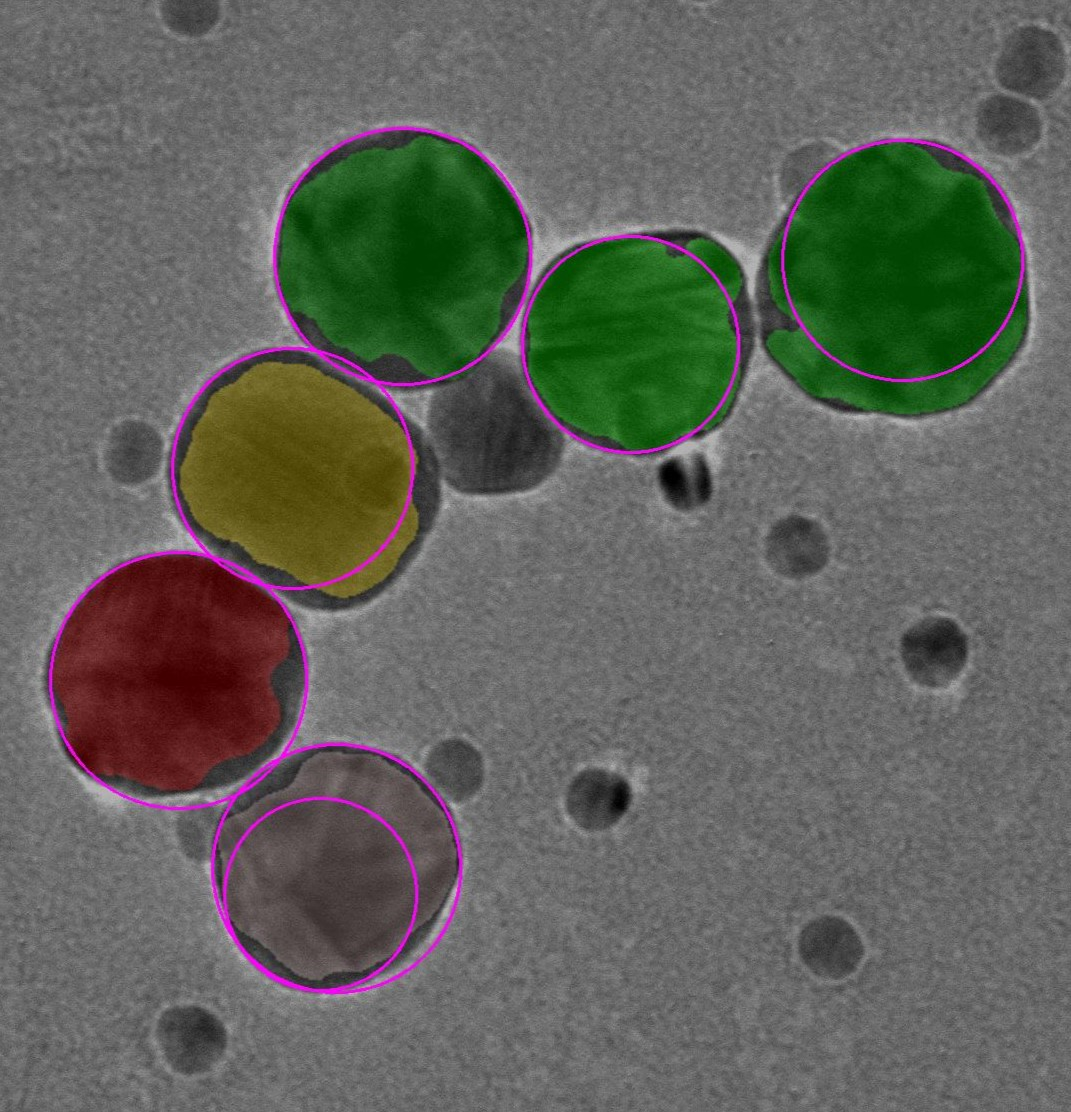
\includegraphics[height=200px]{res40nm.jpg}
\end{subfigure}
\begin{subfigure}(b)
    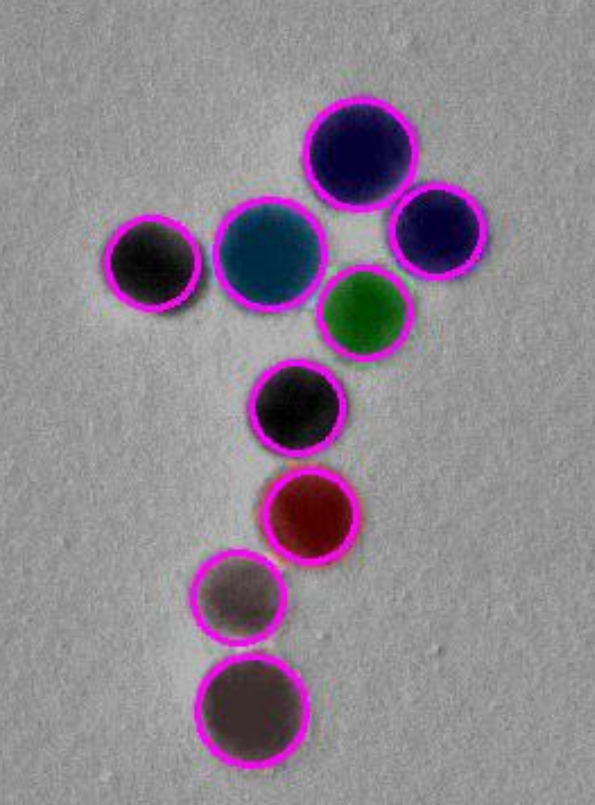
\includegraphics[height=200px]{res50nm.png}
\end{subfigure}
    \caption{Croped result labeled images 40 nm (a) and 50 nm nanoparticles (b)}~\label{fig:res40nm}
\end{center}
\end{figure}

\begin{figure}[h!]
\begin{center}
\begin{subfigure}(a)
    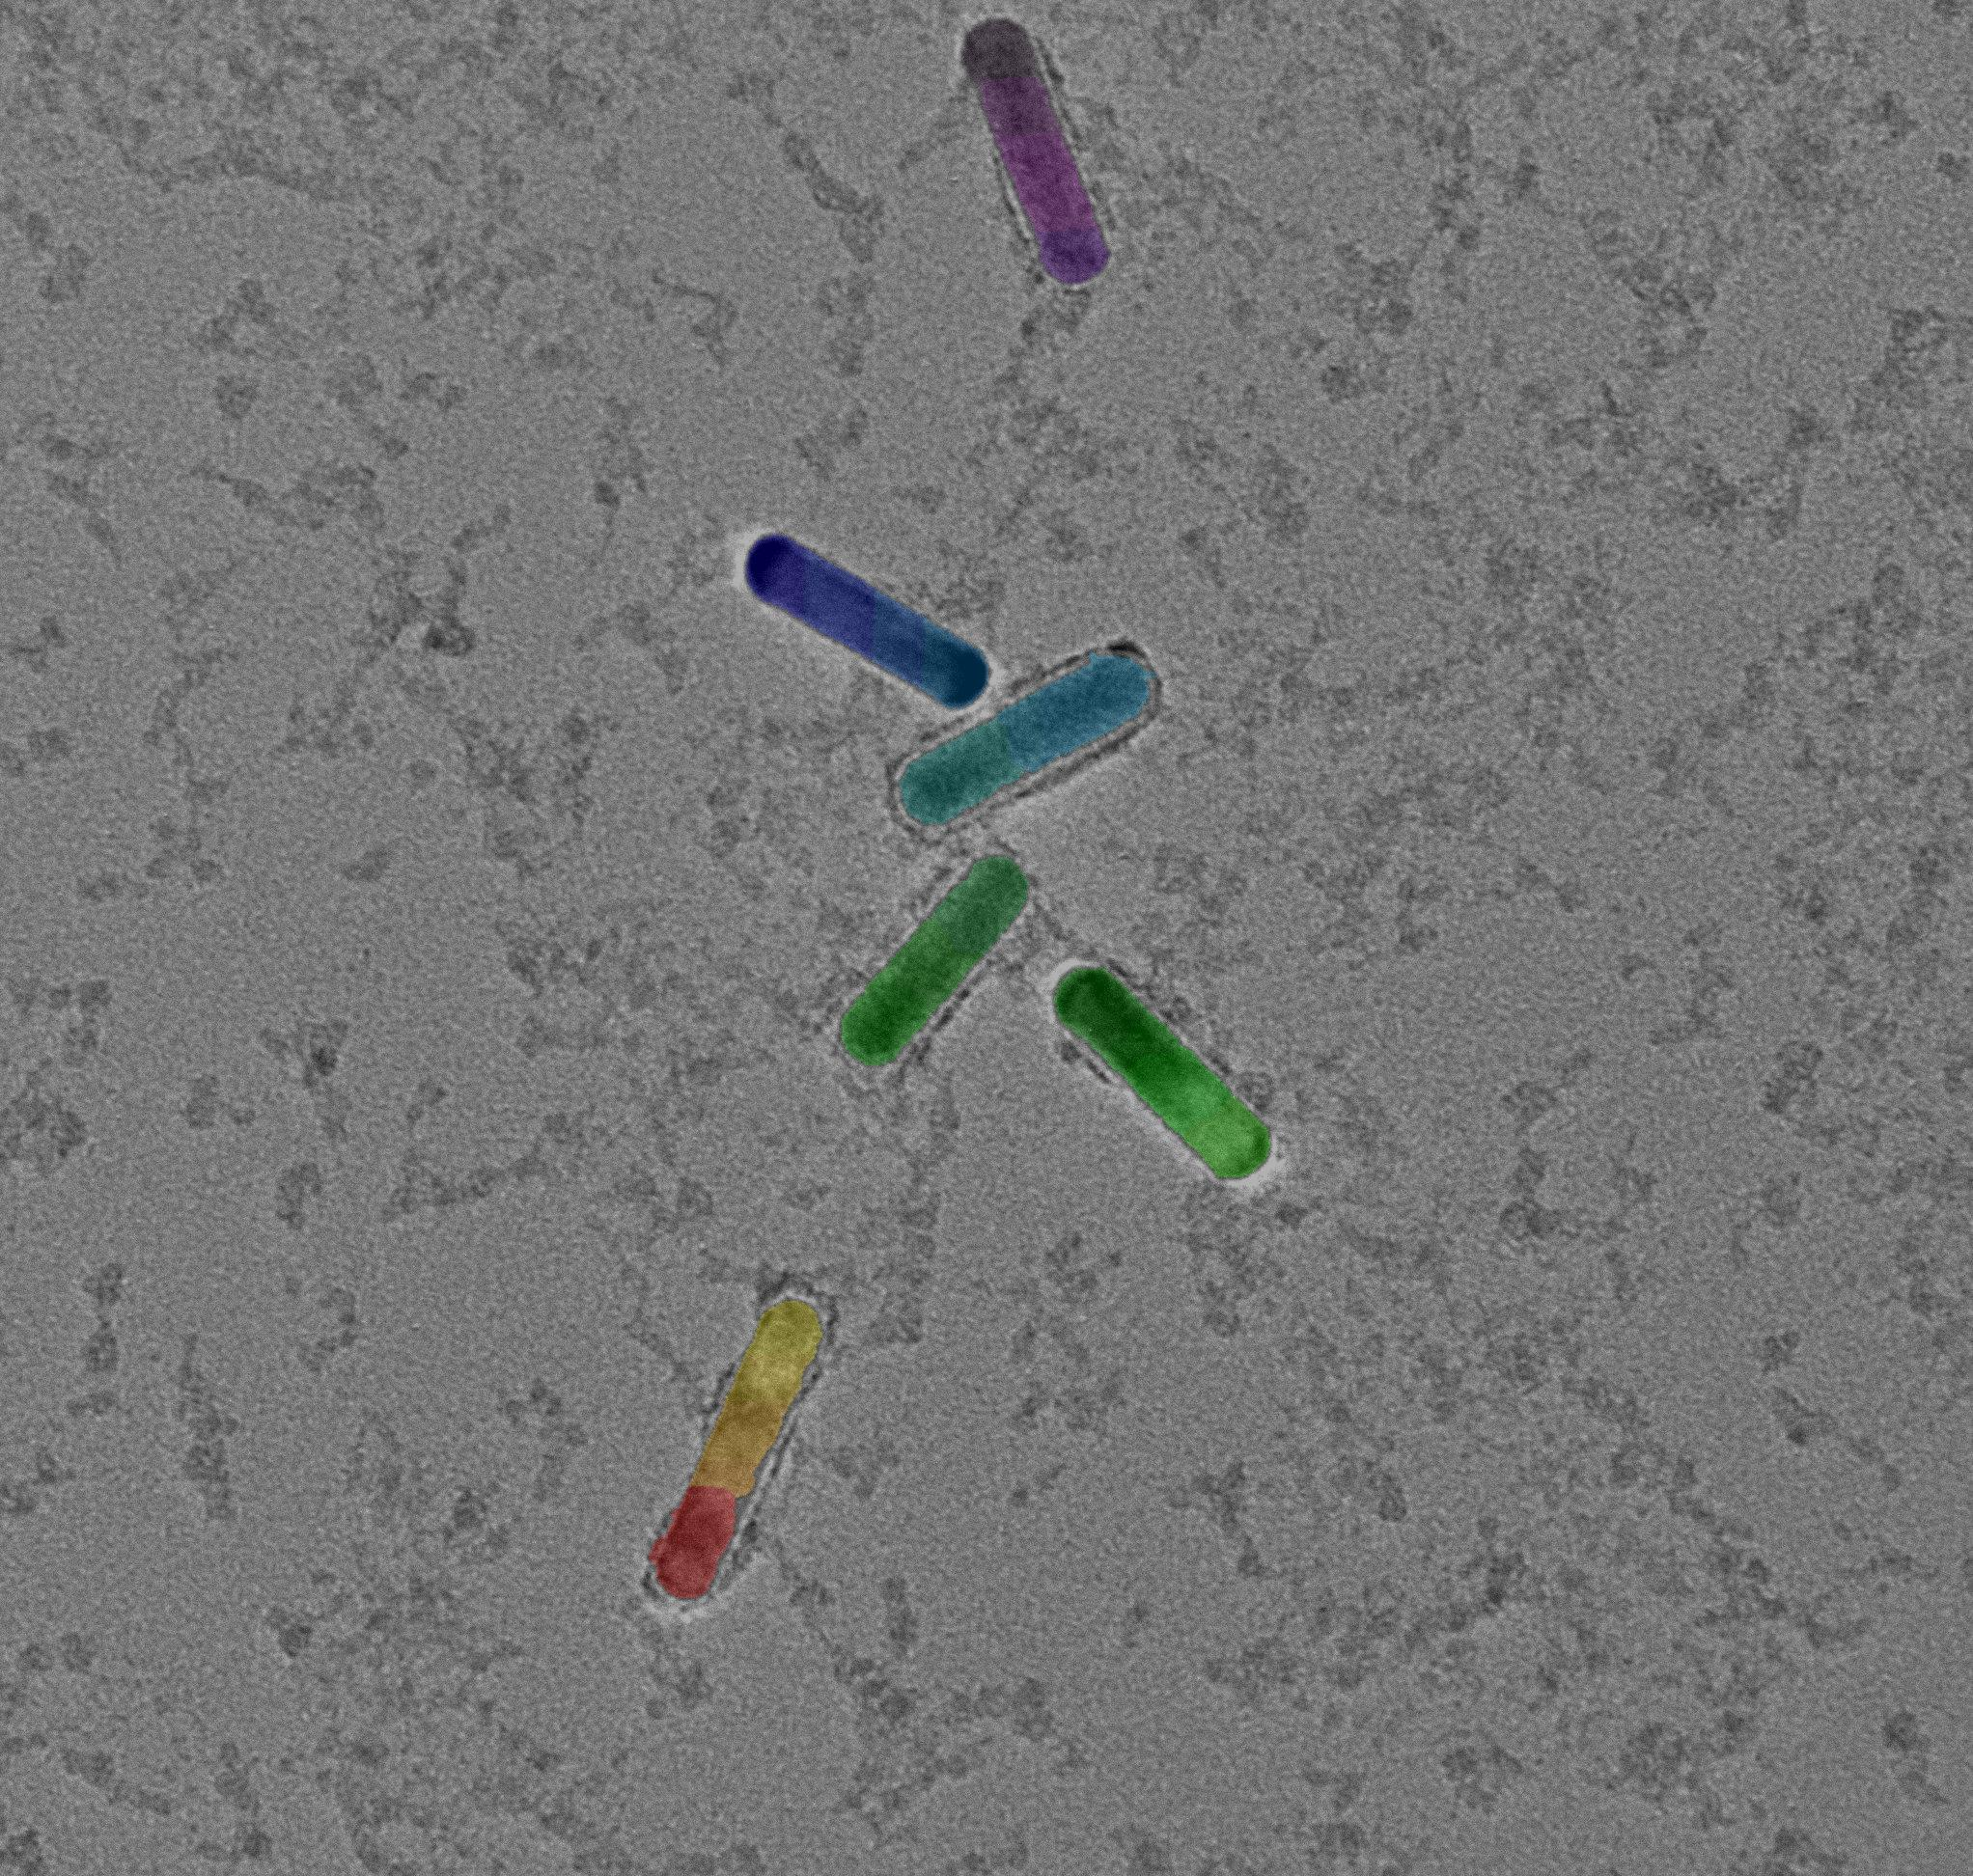
\includegraphics[width=0.4\linewidth]{resNRs.jpg}
\end{subfigure}
\begin{subfigure}(b)
    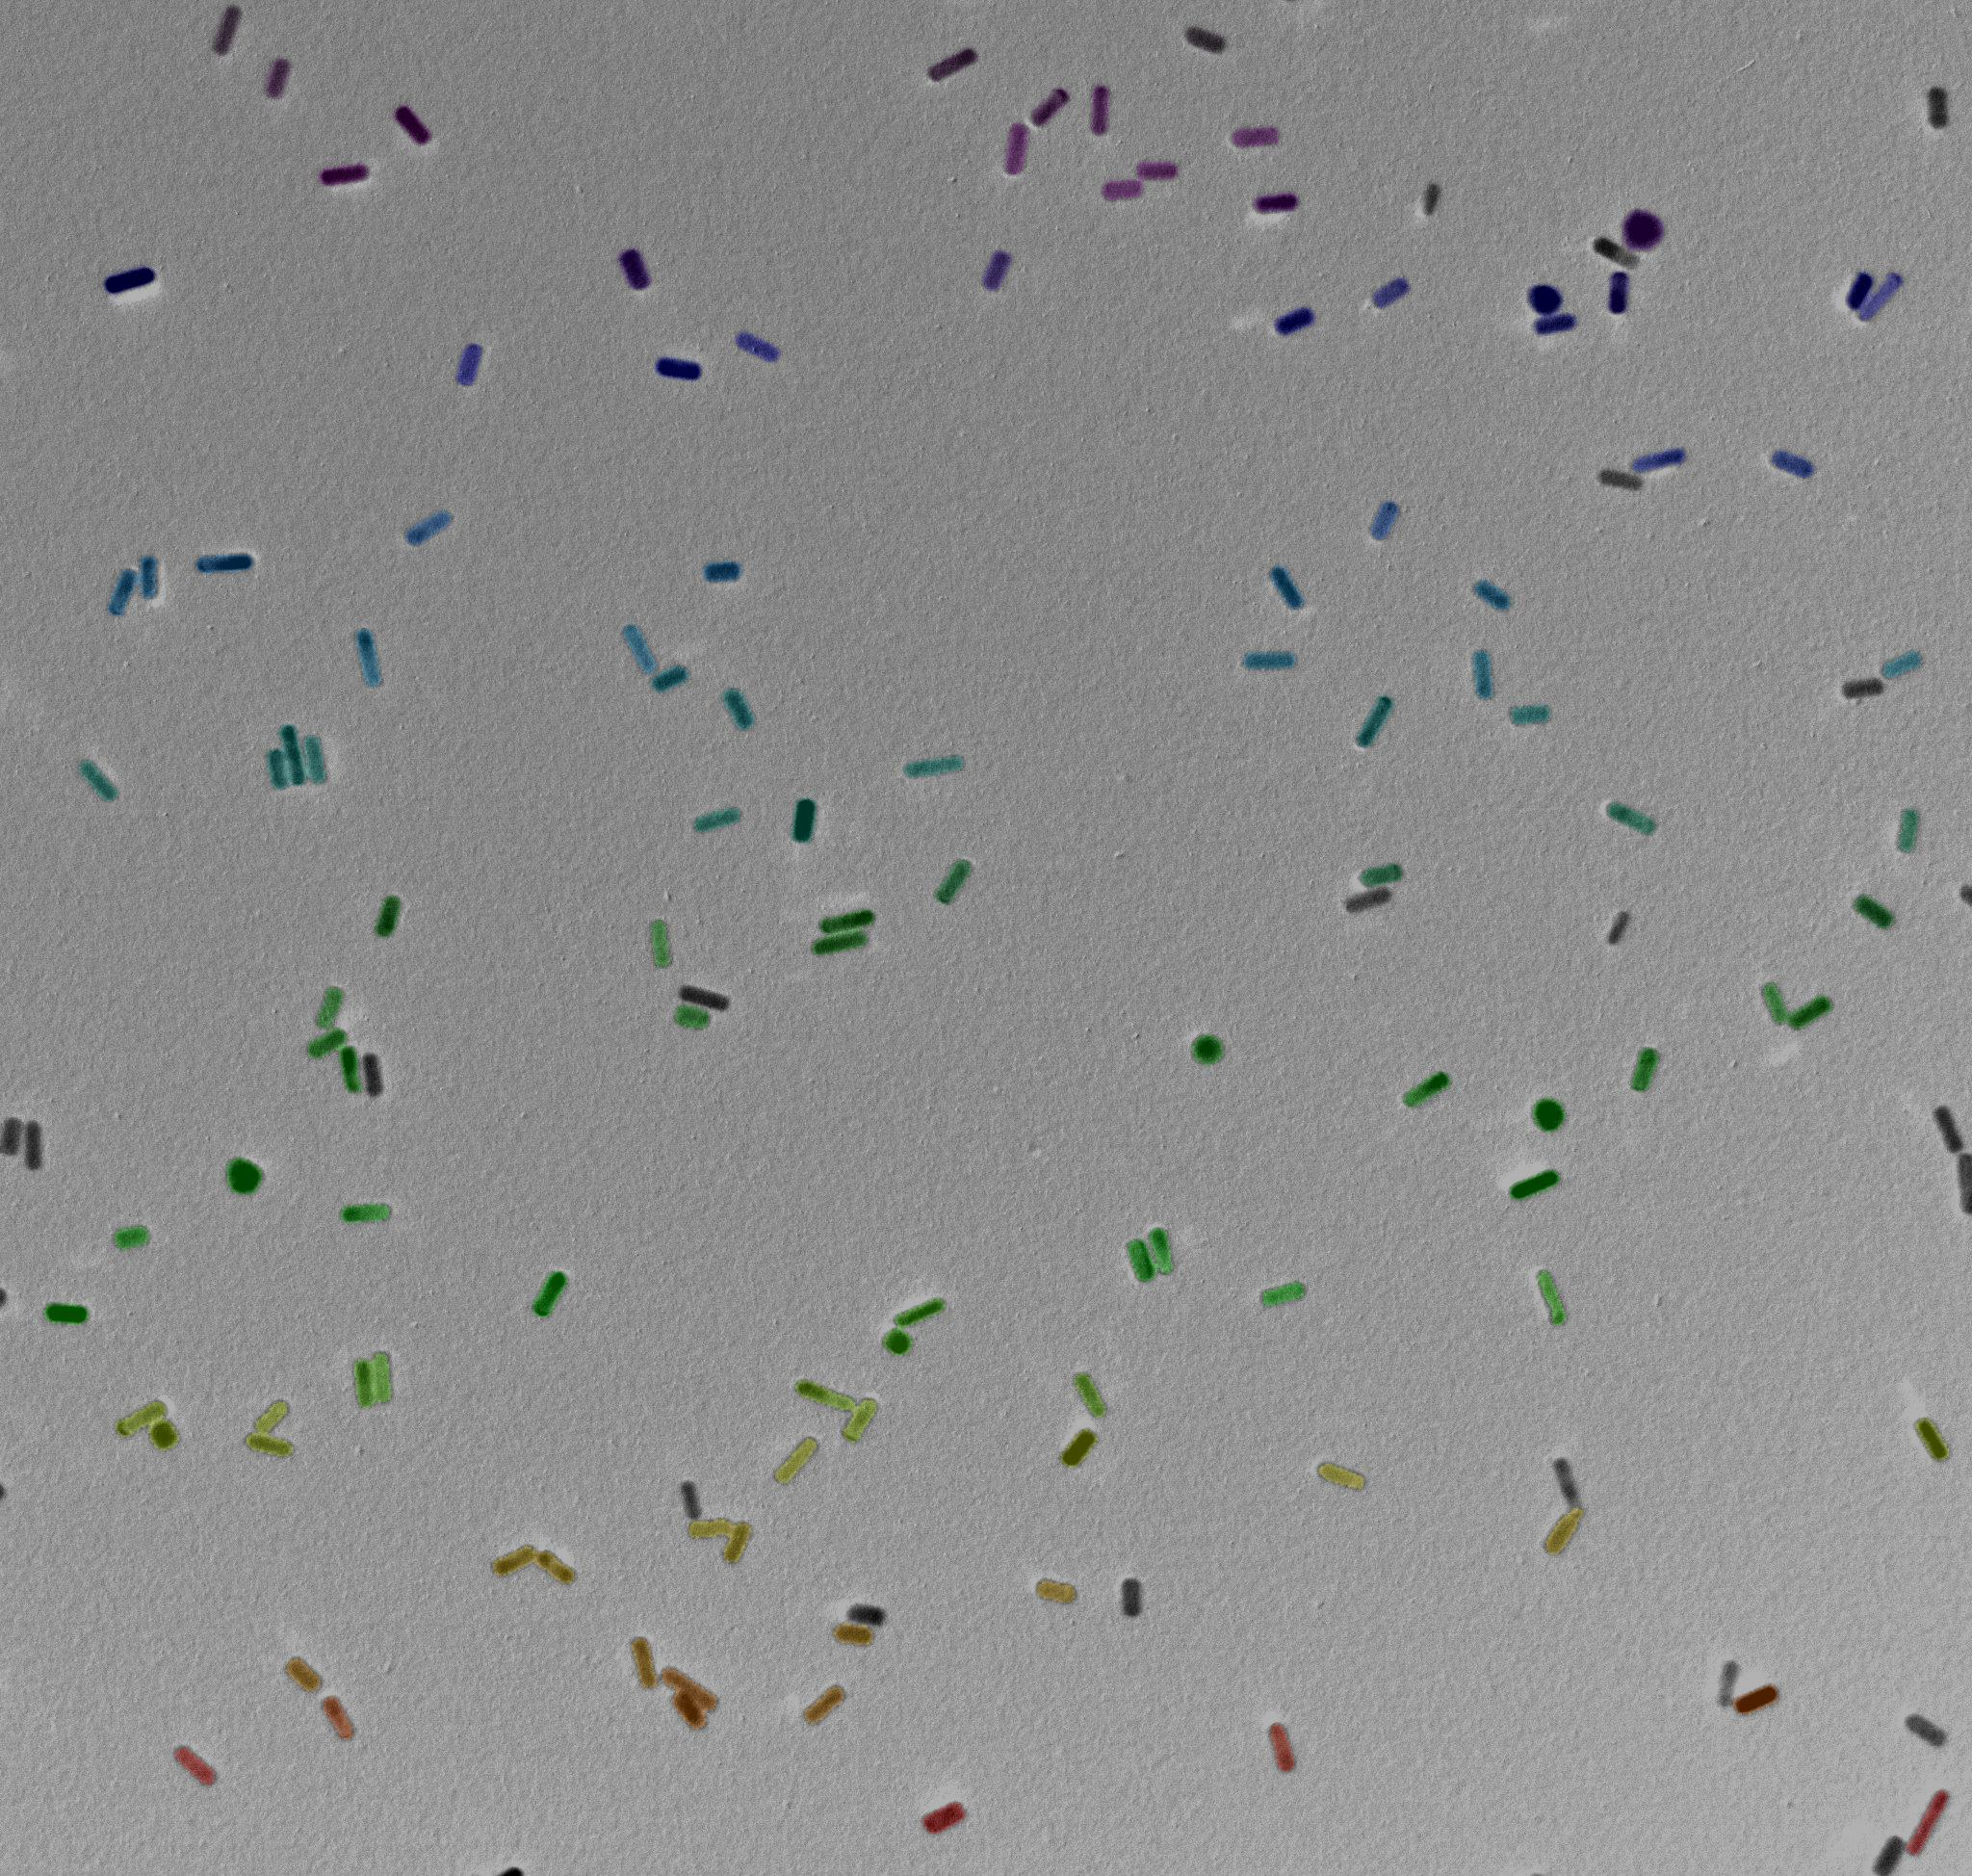
\includegraphics[width=0.4\linewidth]{resNRs2.jpg}
\end{subfigure}
    \caption{Result labeled image on nanorods with absorption peak on 800 nm (a) and 660 nm (b)}~\label{fig:resNRs}
\end{center}
\end{figure}

Histograms of sizes were calculated and plotted, histogram of nanoparticles shows layout of diameters in input image (fig:\ref{fig:hist20nm}) and histogram of nanorods shows major and minor axis lengths in input image (fig:\ref{fig:histNRs}).

\begin{figure}[h!]
\begin{center}
    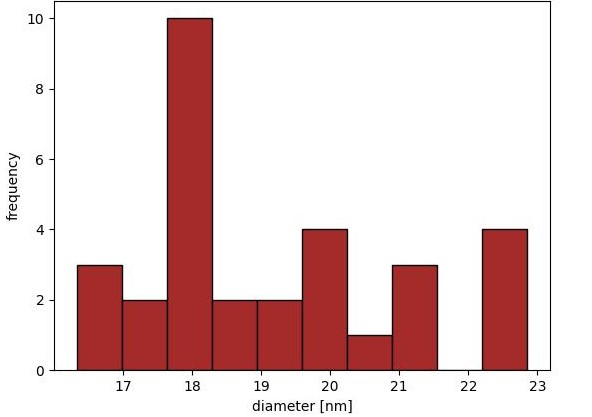
\includegraphics[width=0.8\linewidth]{hist20nm.jpg}
    \caption{Histogram of sizes of 20 nm nanoparticles}~\label{fig:hist20nm}
\end{center}
\end{figure}

\begin{figure}[h!]
\begin{center}
    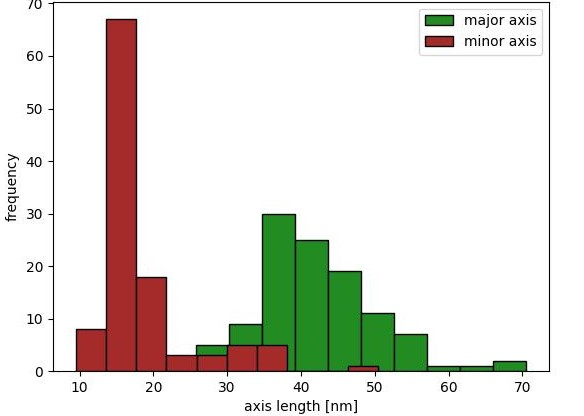
\includegraphics[width=0.8\linewidth]{histNRs.jpg}
    \caption{Histogram of sizes of nanorods with absorption peak on 660 nm}~\label{fig:histNRs}
\end{center}
\end{figure}